\documentclass[aspectratio=169]{beamer}

% ==================================================================
% Define custom colors
\definecolor{primarycolor}{RGB}{25, 74, 166} % blue
\definecolor{accentcolor}{RGB}{65, 155, 232} % lighter blue
\definecolor{bluepoli}{RGB}{2, 30, 54}
\newcommand{\highlight}[2]{\colorbox{#1!9}{$#2$}}

% ==================================================================
% Apply these colors
\setbeamercolor{normal text}{fg=black, bg=white}
\setbeamercolor{alerted text}{fg=accentcolor}
\setbeamercolor{example text}{fg=accentcolor!80!black}
\setbeamercolor{progress bar}{fg=accentcolor, bg=accentcolor!20}
\setbeamercolor{frametitle}{bg=bluepoli, fg=bluepoli!80!black}
\setbeamercolor{title separator}{fg=bluepoli}

% ==================================================================
% Metropolis customization
\usetheme[sectionpage=none]{metropolis}
\setbeamercolor{background canvas}{bg=black!1.5}
\setbeamercolor{frametitle}{bg=black!1.5,fg=black}
\setbeamertemplate{sections/subsections in toc}[square]
\setbeamertemplate{footline}{
    \centerline{\textcolor{bluepoli}{\rule{0.95\paperwidth}{.3pt}}}
    \vskip2.5pt
    \hskip15pt \tiny Root Finding \hskip380pt \insertframenumber
    \vskip4pt
}

% ==================================================================
% Math packages
\usepackage{amsmath}
\usepackage{amssymb}
\usepackage{booktabs}

% ==================================================================
% Images
\usepackage{graphicx}

% ==================================================================
% Colors
\usepackage{color}
\usepackage[dvipsnames]{xcolor}
\usepackage{colortbl}

% ==================================================================
% Code rendering
\usepackage{minted}

% ==================================================================
% TIKZ
\usepackage{tikz}
\usetikzlibrary{positioning,tikzmark,backgrounds,arrows,shapes,calc}

% ==================================================================
% TITLE
\title{Root Finding}
\subtitle{Calcoli di Processo dell'Ingegneria Chimica}
\author[Dinelli]{\textbf{Timoteo~Dinelli}}
\institute{
   Department of Chemistry, Materials and Chemical Engineering, ``Giulio Natta''\\ 
   Politecnico di Milano\\
   \vspace{0.3cm}
   \textbf{email}: timoteo.dinelli@polimi.it
}
\date{October 30\textsuperscript{th}, 2025}

\begin{document}
{
    \setbeamertemplate{footline}{} 
    \begin{frame}{}
        \maketitle
        \begin{tikzpicture}[overlay, remember picture]
            \node[above left=3.6cm and 0.01cm of current page.south east]{
\includegraphics[trim=1cm 1cm 5.5cm 1cm, clip=true, width=8cm]{figures/logo.pdf}};
        \end{tikzpicture}
    \end{frame}
}

% ==================================================================
% Slides
\begin{frame}{Root Finding}
    \begin{columns}
        \column{0.5\textwidth}
            We will discuss different general algorithms that seek to find the solution $\mathbf{x}$ of the following canonical equation:
            \begin{equation*}
                \highlight{accentcolor}{f(\mathbf{x}) = 0}
            \end{equation*}
            
            \vspace{1em}
            \small
            \textcolor{accentcolor}{\textbf{Key concepts:}}
            \begin{itemize}
                \item[$\blacktriangleright$] Iterative approaches
                \item[$\blacktriangleright$] Convergence criteria
                \item[$\blacktriangleright$] Numerical precision
            \end{itemize}
            
        \column{0.5\textwidth}
            \begin{figure}
            \centering
                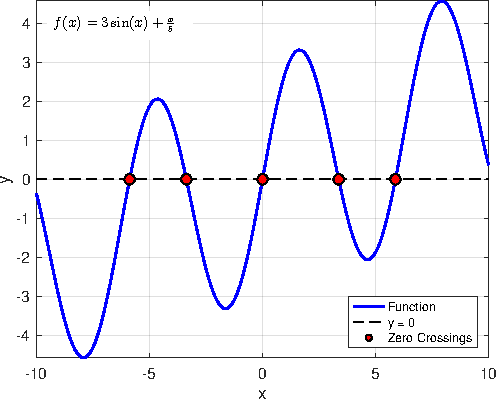
\includegraphics[width=0.95\textwidth]{figures/roots.pdf}
            \end{figure}
    \end{columns}
\end{frame}

\begin{frame}{General Strategy}
    Given the equation:
    \begin{equation*}
        \highlight{accentcolor}{f(\mathbf{x}) = 0}
    \end{equation*}
    
    \vspace{0.5em}
    
    \begin{enumerate}
        \item Make a reasonable first guess $x_{0}$ (or first guesses $x_0$, $x_1$)
            
        \item Test the value of $f(x_{0})$
            
        \item Make a new \alert{intelligent} guess based on $x_{0}$ and $f(x_{0})$
            
        \item Repeat until convergence criteria are met:
        
        \vspace{0.3em}
        \begin{columns}[t]
            \column{0.48\textwidth}
            \textcolor{accentcolor}{\textbf{Function precision:}}
            \begin{equation*}
                \left\lVert f(x_{i+1}) \right\rVert < \epsilon_{f}
            \end{equation*}
            
            \column{0.48\textwidth}
            \textcolor{accentcolor}{\textbf{Solution convergence:}}
            \begin{equation*}
                \left\lVert x_{i+1} - x_{i} \right\rVert < \epsilon_{x}
            \end{equation*}
        \end{columns}
    \end{enumerate}
\end{frame}

\begin{frame}{Bisection Method}
    \textcolor{accentcolor}{\textbf{Theoretical foundation:}}
    
    \small
    Under Bolzano's theorem, if a function $f(x)$ is continuous in the interval $[a, b]$ and takes values of opposite sign at the boundaries, then it has a root in that interval.
    
    \vspace{0.5em}
    
    \normalsize
    \textcolor{accentcolor}{\textbf{Algorithm:}}
    
    \small
    Starting with interval $[a, b]$, function $f(x)$, and tolerance $\epsilon$ such that $\|c - \hat{c}\| < \epsilon$, where $\hat{c}$ is the root:
    
    \vspace{0.3em}
    
    \begin{enumerate}
        \item Compute midpoint: $c = \dfrac{a+b}{2}$
            
        \item If $b-c \leq \epsilon$, then $c$ is the solution — stop; otherwise, continue
            
        \item If $\text{sign}(f(b)) \times \text{sign}(f(c)) \leq 0$, then $a = c$; else $b = c$
        
        \item Return to step 1 and repeat
   \end{enumerate}
\end{frame}

\begin{frame}{Newton's Method}
    \textcolor{accentcolor}{\textbf{Algorithm:}}
    
    \begin{enumerate}
        \item Make a reasonable first guess $x_{0}$
        
        \item Compute the next guess using:
        \begin{equation*}
            \highlight{accentcolor}{x_{i+1} = x_{i} - \frac{f(x_{i})}{f'(x_{i})}}
        \end{equation*}
        
        \item Repeat until required precision is reached
    \end{enumerate}
    
    \vspace{1em}
    \centering
    \alert{\textbf{Challenge:}} How do we compute $f'(x_{i})$?
\end{frame}

\begin{frame}{Computing Derivatives}
    \begin{columns}
        \column{0.48\textwidth}
        \textcolor{accentcolor}{\textbf{Classical Analysis:}}
        \begin{equation*}
            f'(x_{0}) = \lim_{h \to 0}\frac{f(x_{0} + h) - f(x_{0})}{h}
        \end{equation*}
        
        \vspace{1em}
        Exact mathematical definition using limits
        
        \column{0.48\textwidth}
        \textcolor{accentcolor}{\textbf{Numerical Analysis:}}
        \begin{equation*}
            f'(x_{0}) \approx \frac{f(x_{0} + h) - f(x_{0})}{h}
        \end{equation*}
        
        \vspace{1em}
        Pick a small value for $h$\\
        (e.g., $h = 1 \times 10^{-7}$)
    \end{columns}
    
    \vspace{1em}
    \begin{center}
    \textcolor{primarycolor}{\small\textit{Finite difference approximation enables practical computation}}
    \end{center}
\end{frame}

\begin{frame}{Secant Method}
   \small
   The Newton method simplifies $f(x) = 0$ using the tangent as an approximation. The \alert{secant method} uses a secant line instead, requiring two initial guesses.
   
   \vspace{0.5em}
   
   \textcolor{accentcolor}{\textbf{Algorithm:}}
   
   Assuming we know $f(x)$ for two distinct values $x_0$ and $x_1$ close to the solution $\alpha$:
   
   \vspace{0.3em}
    \begin{enumerate}
        \item Make reasonable first guesses $x_{0}$ and $x_{1}$
        
        \item Compute $f(x_0)$ and $f(x_1)$, then calculate:
        \begin{equation*}
            x_2 = x_1 - \frac{f(x_1)(x_1 - x_0)}{f(x_1) - f(x_0)}
        \end{equation*}
        
        \item Loop until convergence
    \end{enumerate}

    \vspace{0.1em}
    \textcolor{accentcolor}{\textbf{General iterative formula:}}
    \begin{equation*}
        \highlight{accentcolor}{x_{n+1} = x_{n} - \frac{f(x_{n})(x_n - x_{n-1})}{f(x_n) - f(x_{n-1})}}
    \end{equation*}
\end{frame}

\begin{frame}{Regula Falsi Method}
   \textcolor{accentcolor}{\textbf{Hybrid approach:}} Combines features of bisection and secant methods
   
   \vspace{0.8em}
   
   The \textit{regula falsi} (false position) method:
   \begin{itemize}
       \item[$\blacktriangleright$] Uses secants like the secant method
       \item[$\blacktriangleright$] Maintains an uncertainty interval like bisection
       \item[$\blacktriangleright$] Requires function values of opposite signs at interval boundaries
       \item[$\blacktriangleright$] Guarantees convergence for continuous functions
   \end{itemize}
   
   \vspace{0.8em}
   
   \textcolor{NavyBlue}{\textbf{Key difference from secant:}} The two points always bracket the root, ensuring the solution remains within the interval throughout iterations.
   
   \vspace{0.8em}
   
   \begin{center}
   \small\textit{More robust than secant method, faster than bisection}
   \end{center}
\end{frame}

\begin{frame}{Method Comparison}
    \begin{center}
    \small
    \begin{tabular}{lccc}
        \toprule
        \textbf{Method} & \textbf{Initial Guesses} & \textbf{Convergence Rate} & \textbf{Derivative} \\
        \midrule
        Bisection & 2 (bracketing) & Linear & Not required \\
        Newton & 1 & Quadratic & Required \\
        Secant & 2 (any) & Superlinear & Not required \\
        Regula Falsi & 2 (bracketing) & Superlinear & Not required \\
        \bottomrule
    \end{tabular}
    \end{center}
    
    \vspace{1em}
    
    \textcolor{accentcolor}{\textbf{Selection criteria:}}
    \begin{itemize}
        \item[$\blacktriangleright$] \textbf{Newton:} Fastest when derivative is easily computed
        \item[$\blacktriangleright$] \textbf{Secant:} Good balance when derivative is costly
        \item[$\blacktriangleright$] \textbf{Bisection:} Most robust, guaranteed convergence
        \item[$\blacktriangleright$] \textbf{Regula Falsi:} Combines robustness with better speed
    \end{itemize}
\end{frame}

{
    \setbeamertemplate{footline}{}
    \begin{frame}[standout]
        Exercises
    \end{frame}
}

\begin{frame}{Exercise}
    \begin{itemize}
        \item[$\blacktriangleright$]
        Let's implement the \alert{Bisection} and \alert{Newton} method to find the zero of a function. Test them against $f(x) = 3e^{x} - 4cos(x)$.
        
        \item[$\blacktriangleright$]
        (Exam 05/02/19, Exercise 4): Find the root of the function $f(x) = \frac{1}{x-2} - 2$. After several attempts it can be noticed that the Newton method fails for first guesses as $x_{0} = 1.8$ and $x_{0} = 4$, while converge rapidly if the first guess is equal to $x_{0} = 2.2$. Explain why this happens using also a graphical representation, determine the interval where is possible to identify a first guess that allows the method to converge. Compute the solution using Newton method and Bisection method with a precision of $1e^{-2}$. Then compare the results obtained with the Matlab's built-in method \textcolor{blue}{fzero} and \textcolor{blue}{fsolve}.
    \end{itemize}
\end{frame}

\begin{frame}{}
    \begin{figure}
        \centering
        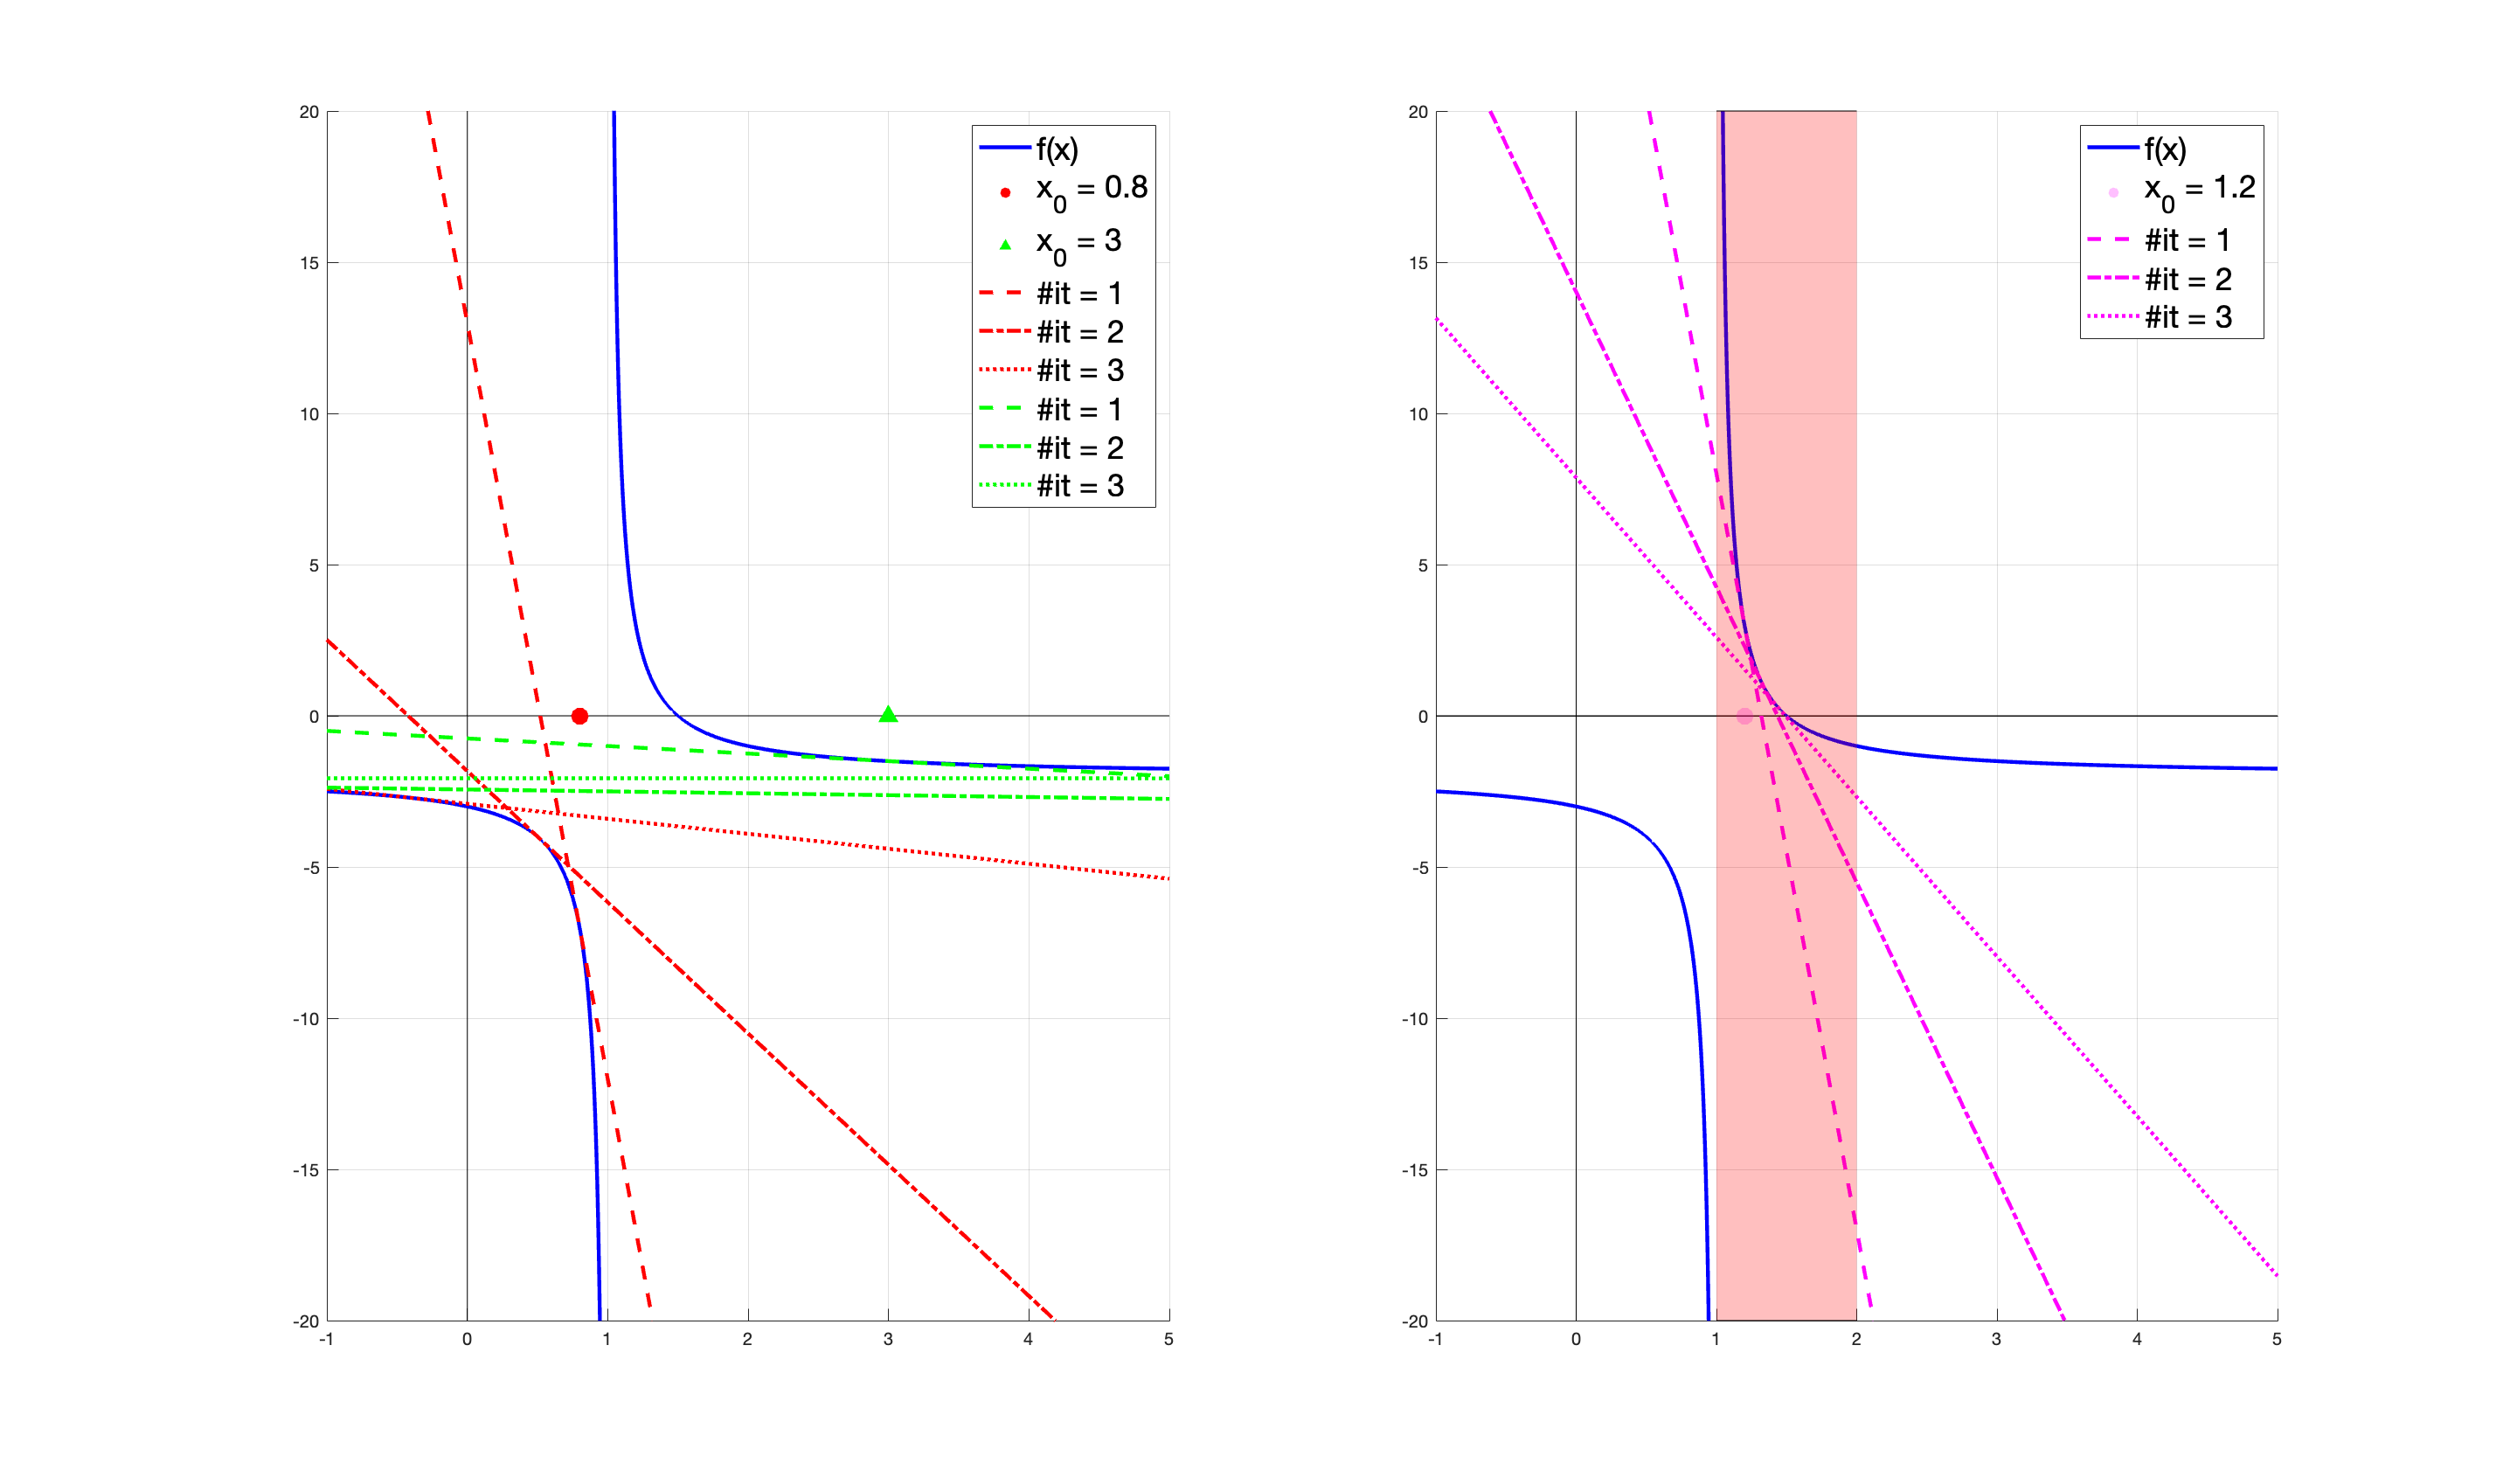
\includegraphics[width=1.\textwidth]{figures/newton_choose.png}
    \end{figure}
\end{frame}

\begin{frame}{}
    \begin{itemize}
        \item[$\blacktriangleright$]
        From the DIPPR\textsuperscript{\textregistered} database we learn that, for WATER ($H_{2}O$), the Vapor Pressure can be calculated In the range 273.16 K to 647.13 K as follows:
        \begin{equation*}
            P^{0}_{vap} (T) = exp\left(A + \frac{B}{T} + C \times ln(T) + D \times T^{E}\right ) \quad [Pa]
        \end{equation*}
         Where: $T$ is the temperature in Kelvin, $A = 7.3649e^{+01}$, $B = -7.2582e^{+03}$, $C = -7.3037e^{+00}$, $D = 4.1653e^{-06}$, $E = 2.0000e^{+00}$. Determine, using the newton method, for which temperature the vapor pressure is 0.5 $atm$
    \end{itemize}
\end{frame}

\begin{frame}{}
    \begin{itemize}
        \item[$\blacktriangleright$]
        Write a function that calculates the bubble temperture of a binary blend of NC6 and NC7 (70/30 molar) at atmospheric pressure using a solver you developed (the solver will be a function that takes the function to be solved, the interval or the first guess needed to start the iterative procedure and the desired precision of the solution and returns the zero of the function. \textbf{Bubble Temperature of a mixture}.
        \begin{equation*}
            \sum_{i=1}^{NS} y_{i} = 1 \longrightarrow y_{i} = \frac{P_{i}^{0}(T)}{P}z_{i}
        \end{equation*}
        \begin{equation*}
            f(x) = 1 - \sum_{i=1}^{NS} \frac{P_{i}^{0}(T_{bubble})}{P}z_{i} = 0
        \end{equation*}
    \end{itemize}
\end{frame}

{
    \setbeamertemplate{footline}{}
    \begin{frame}[standout]
        Thank you for your attention!
    \end{frame}
}
\end{document}